\documentclass{article}
\usepackage{graphicx}
\usepackage{natbib}
\usepackage{hyperref}
\usepackage{setspace}        % for double spacing
\usepackage{tikz}
\usepackage{pgfplots}        % for plots
\pgfplotsset{compat=1.17}
\usepackage{amsmath}          % for advanced math
\DeclareMathOperator{\logit}{logit}   % define logit operator

\title{The Impact of Indian Health Service Budget on Native American Infant Mortality}
\author{Yeganeh Karbalaei}
\date{April 2025}

\begin{document}
\doublespacing
\maketitle

\section{Introduction}
Despite decades of fundamental public health interventions, American Indian and Alaska Native (AIAN) people continue to experience disproportionately high infant mortality rates, even as other racial and ethnic groups in the United States have seen significant improvements. This persistent disparity suggests that structural and systemic factors, beyond individual health behaviors, contribute to differences in infant health outcomes.

This study investigates the causal effect of Indian Health Service (IHS) budget appropriations on infant mortality among AIAN populations. While previous research has explored the medical causes of Native American infant deaths—such as congenital malformations, sudden infant death syndrome (SIDS), and unintentional injuries—there is a considerable lack of research addressing the impact of the healthcare delivery system itself, particularly the role of IHS funding and service provision.

\section{Literature Review}
Infant mortality refers to the death of a baby that occurs between the time it is born and 1~year of age. If a baby dies before age 28~days, the death can also be classified as neonatal mortality \citep{infantmortality}. Infant mortality rate is the number of infant deaths (under one year of age) per 1,000 live births in a given year.

Despite overall improvements in decreasing infant mortality rates (IMR) in the United States, significant racial disparities persist. A recent review by \citet{jang_review_2022} finds the U.S. overall IMR was 5.58 per 1,000 live births in 2018, but non--Hispanic Black infants experienced 10.8, Native Hawaiian/Pacific Islanders 9.4, and American Indian infants 8.2—more than 70\% higher than the non--Hispanic White rate of 4.6 \citep{jang_review_2022}. However, overall all ethnicities except Native American have experienced a decline in IMR in recent 30 years.  Between 2005 and 2014, while other racial and ethnic groups saw steady declines, the American Indian IMR showed no significant improvement—a pattern confirmed in Alaska, where AIAN infants’ IMR averaged 9.3 between 2016 and 2018 \citep{jang_review_2022,the_university_of_arizona_whats_2017}.

Linkage of National Vital Statistics and IHS registration records reveals that from 1999--2009, AIAN infants died at a rate of 9.14 per 1,000 live births, with elevated proportions of deaths due to SIDS, unintentional injuries, influenza, and pneumonia \citep{wong_american_2014}. Indeed, the overall AIAN SIDS death rate remains more than double that of non--Hispanic whites \citep{macdorman_m_f_understanding_2011}. Congenital malformations, short gestation and low birth weight, and unintentional injuries also rank among the leading causes of death for AIAN infants \citep{wong_american_2014}.

Parental health behaviors further compound risk: smoking rates among Native American women are nearly twice those of other groups in states like Alaska and Minnesota, contributing to low birth weight and preterm births \citep{kaplan1997prevalence}. 

Although the Indian Health Service (IHS) has provided free services since 1955, funding shortages have forced many AIAN families onto Medicaid or private plans. Medicaid covers over 25\% of nonelderly AIAN adults and 50\% of AIAN children, yet more than 900,000 Native Americans remain uninsured \citep{samantha_artiga_medicaid_2017}. Chronic under--funding of IHS—currently meeting only about 60\% of estimated need—has left many service units understaffed and facilities outdated, directly contributing to the perinatal and infant health disparities observed across tribal communities \citep{ASPE2022,WarneFrizzell2014}.

\section{Data}
I used CDC Linked Birth--Infant Death data (2000--2005), budget of Indian Health Service from United States Department of Health and Human Services annual budget report, and annual health inflation from Bureau of Labor Statistics. 

\section{Methods}
We estimate the following logistic regression model:
\begin{align}
\logit\bigl(P(\mathrm{InfantDeath}_{i}=1)\bigr)
&= \beta_{0} + \beta_{1}\,\mathrm{IHSBudget}_{c,t} + \beta_{2}\,\mathrm{PrenatalVisits}_{i} + \beta_{3}\,\mathrm{BirthWeight}_{i}
\notag\\
&\quad + \beta_{4}\,\mathrm{GestationalAge}_{i} + \beta_{5}\,\mathrm{Congenital}_{i} + \beta_{6}\,\mathrm{MotherAge}_{i} + \gamma_{t} + \delta_{c}.
\label{eq:logit}
\end{align}

\section{Findings}
I analyzed 42552 infants who were born from native American mothers or fathers during 2000-2002. Preliminary results indicate that higher IHS budgets per county is associated with lower odds of infant mortality. However, the result I got shows it is marginally significant. Surprisingly, the coefficient of prenatal visits is positive, meaning that each additional prenatal visit is associated with a 0.0056 unit increase in log odds of infant death. As I expected, each extra gram of birth weight reduces the logarithmic odds of dying by 0.00147 (OR≈ 0.9985 per gram, or approximately a 1. 5\% drop in the odds per 100 g). This is highly significant. Also, Each additional week of gestation reduces log‐odds of death by 0.05 and it is highly significant. The only mother characteristic I used in this model was age. Similar to previous studies, older maternal age appears slightly protective, significant at the 5\% level.

\section{Conclusion}
Although, the coefficient of IHS budget index is not significantly associated with reduction of log-odds of infant death by adding more control variables especially geographical data, the result may change. Also, I just used small numbers of records to find out the challenges of cleaning and coding. For further steps, I will include more observations.  
Regarding prenatal visits variable and how it is associated with infant death, I did not expect to have positive coefficient. However, it showed that there is an endogenity problem as probably high-risk mothers had prenatal care visits more than mothers with standard health condition. Also, their infants have higher risk of death before their first birthdays. 

\newpage
\section*{Figures}
\begin{itemize}
    \item % Placeholder for prenatal visits graph
Here a graph will be inserted to show the number of prenatal visits among different races.
     \item infant mortality graph
     % Infant mortality rates over time
\begin{figure}[h]
  \centering
  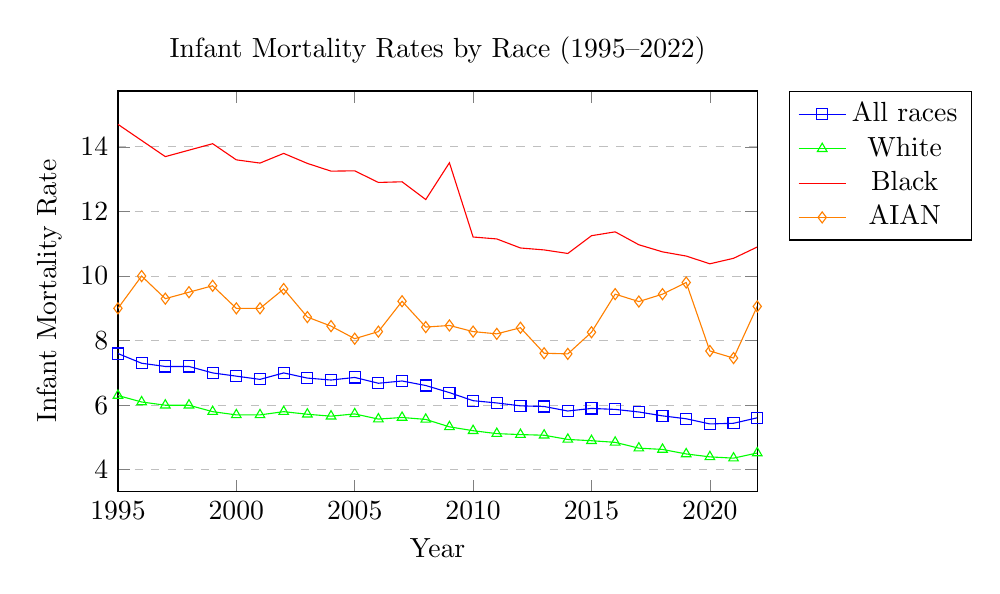
\begin{tikzpicture}
    \begin{axis}[
      width=0.8\textwidth,
      height=0.55\textwidth,
      xlabel={Year},
      ylabel={Infant Mortality Rate},
      title={Infant Mortality Rates by Race (1995--2022)},
      xmin=1995, xmax=2022,
      xtick={1995,2000,2005,2010,2015,2020},
      xticklabels={1995,2000,2005,2010,2015,2020},
      tick label style={font=\normalsize},
      label style={font=\normalsize},
      title style={font=\normalsize},
      legend pos=outer north east,
      legend style={at={(1.05,1)},anchor=north west,font=\normalsize},
      ymajorgrids=true,
      grid style=dashed,
    ]
      \addplot[color=blue,mark=square] coordinates {
        (1995,7.6) (1996,7.3) (1997,7.2) (1998,7.2) (1999,7.0)
        (2000,6.9) (2001,6.8) (2002,7.0) (2003,6.84) (2004,6.78)
        (2005,6.86) (2006,6.68) (2007,6.75) (2008,6.61) (2009,6.39)
        (2010,6.14) (2011,6.07) (2012,5.98) (2013,5.96) (2014,5.82)
        (2015,5.90) (2016,5.87) (2017,5.79) (2018,5.67) (2019,5.58)
        (2020,5.42) (2021,5.44) (2022,5.61)
      }; \addlegendentry{All races}
      \addplot[color=green,mark=triangle] coordinates {
        (1995,6.3) (1996,6.1) (1997,6.0) (1998,6.0) (1999,5.8)
        (2000,5.7) (2001,5.7) (2002,5.8) (2003,5.72) (2004,5.66)
        (2005,5.73) (2006,5.57) (2007,5.62) (2008,5.56) (2009,5.33)
        (2010,5.21) (2011,5.12) (2012,5.09) (2013,5.07) (2014,4.94)
        (2015,4.90) (2016,4.85) (2017,4.67) (2018,4.63) (2019,4.49)
        (2020,4.40) (2021,4.36) (2022,4.52)
      }; \addlegendentry{White}
      \addplot[color=red,mark=circle] coordinates {
        (1995,14.7) (1996,14.2) (1997,13.7) (1998,13.9) (1999,14.1)
        (2000,13.6) (2001,13.5) (2002,13.8) (2003,13.49) (2004,13.25)
        (2005,13.26) (2006,12.9) (2007,12.92) (2008,12.37) (2009,13.51)
        (2010,11.21) (2011,11.15) (2012,10.87) (2013,10.81) (2014,10.70)
        (2015,11.25) (2016,11.37) (2017,10.97) (2018,10.75) (2019,10.62)
        (2020,10.38) (2021,10.55) (2022,10.90)
      }; \addlegendentry{Black}
      \addplot[color=orange,mark=diamond] coordinates {
        (1995,9.0) (1996,10.0) (1997,9.3) (1998,9.5) (1999,9.7)
        (2000,9.0) (2001,9.0) (2002,9.6) (2003,8.73) (2004,8.45)
        (2005,8.06) (2006,8.28) (2007,9.22) (2008,8.42) (2009,8.47)
        (2010,8.28) (2011,8.21) (2012,8.40) (2013,7.61) (2014,7.59)
        (2015,8.26) (2016,9.44) (2017,9.21) (2018,9.44) (2019,9.80)
        (2020,7.68) (2021,7.46) (2022,9.06)
      }; \addlegendentry{AIAN}
    \end{axis}
  \end{tikzpicture}
  \caption{Infant Mortality Rates by Race in the United States (1995--2022)}
  \label{fig:infant_mortality}
\end{figure}

  \item graph of IHS budget change 
\end{itemize} 



\newpage
\section*{Tables}
\begin{table}[ht]
\centering
\caption{Logit Estimates of Infant Death}
\label{tab:logit}
\begin{tabular}{lccc}
\toprule
 & Estimate & Std.\ Error & $p$-value \\
\midrule
Intercept                     & 2.766    & 1.201      & 0.0213$^{*}$ \\
IHS Budget Index              & $-0.02199$ & 0.01296    & 0.0897 \\
Prenatal Visits               & 0.005653 & 0.002002   & 0.00475$^{**}$ \\
Birth Weight (g)              & $-0.001467$ & 0.0000957  & $<0.001^{***}$ \\
Gestational Age (weeks)       & $-0.04984$ & 0.01614    & 0.00201$^{**}$ \\
Mother Age                    & $-0.02146$ & 0.008835   & 0.0152$^{*}$ \\
Year = 2001                   & 0.12297  & 0.1795     & 0.4933 \\
Year = 2002                   & 0.10687  & 0.1802     & 0.5532 \\
\addlinespace
\multicolumn{4}{l}{\textit{County fixed effects included (omitted for brevity).}}\\
\midrule
Observations                  & \multicolumn{3}{c}{42552}  \\
McFadden’s pseudo $R^2$       & \multicolumn{3}{c}{0.274}  \\
\bottomrule
\end{tabular}

\begin{flushleft}
\tiny Notes: $^{*}p<0.05,\;^{**}p<0.01,\;^{***}p<0.001$.  Standard errors in parentheses.
\end{flushleft}
\end{table}

\bibliographystyle{apalike}
\bibliography{PS11_Karbalaei}

\end{document}



